\setlength{\columnsep}{3pt}
\begin{flushleft}
	\textbf{setfacl}: Used to add a new ACL rule or modify an existing rule on a file or directory.
	\newline
	Syntax for ACL rule on user:
	\begin{tcolorbox}[breakable,notitle,boxrule=-0pt,colback=pink,colframe=pink]
		\color{black}
		\fontdimen2\font=9pt
		Syntax: setfacl -m u:user\_name:permissions file\_or\_directory
		\fontdimen2\font=4pt
	\end{tcolorbox}
	
	Syntax for ACL rule on group:
	\begin{tcolorbox}[breakable,notitle,boxrule=-0pt,colback=pink,colframe=pink]
	\color{black}
	\fontdimen2\font=0.5em
	Syntax: setfacl -m g:group\_name:permissions file\_or\_directory
	\fontdimen2\font=4pt
	\end{tcolorbox}

	\item Eg: Apply ACL rule on directory \textbf{project}, such as:
	\begin{itemize}
		\item User named \textbf{John} should have read, write and execute permission
		\item User named \textbf{Jimmy} should have read and execute permission
		\item Group named \textbf{managers} should have read, write and execute permission
		\item Group named \textbf{testers} should have read and execute permission
	\end{itemize}
	\bigskip

	\begin{tcolorbox}[breakable,notitle,boxrule=-0pt,colback=black,colframe=black]
		\color{green}
		\fontdimen2\font=9pt
		\# setfacl -m u:John:rwx,u:Jimmy:r-x project
		\newline
		\# setfacl -m g:managers:rwx,g:testers:r-x project
		\fontdimen2\font=4pt
	\end{tcolorbox}
\newpage
	
	\bigskip
	\textbf{getfacl}: Used to check ACL rules applied directory or files.
	\begin{tcolorbox}[breakable,notitle,boxrule=-0pt,colback=pink,colframe=pink]
		\color{black}
		\fontdimen2\font=9pt
		Syntax: getfacl  file\_or\_directory
		\fontdimen2\font=4pt
	\end{tcolorbox}
	Eg:
	\begin{figure}[h!]
		\centering
		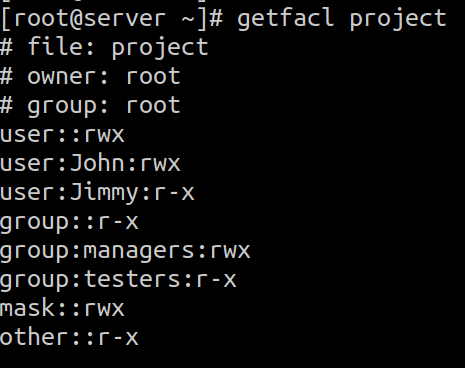
\includegraphics[scale=0.6]{content/chapter6/images/getfacl.png}
		\caption{Sample output}
		\label{fig:getfacl}
	\end{figure}
	
	
\newpage

\textbf{Default ACL rules}: 
\begin{itemize}
	\item \textbf{For directories, you can set ACL rules that will be assigned by defaults} to files and directories created inside it. 
	\item To do so, use the default identificator using \textbf{-R} option and \textbf{d} character in setfacl command.
	\item Syntax for default ACL rule for user:
	\bigskip
	\begin{tcolorbox}[breakable,notitle,boxrule=-0pt,colback=pink,colframe=pink]
		\color{black}
		\fontdimen2\font=0.5em
		Syntax: setfacl -R -m d:u:user\_name:permissions directory
		\fontdimen2\font=4pt
	\end{tcolorbox}

	\item Syntax for default ACL rule for group:
	\bigskip
	\begin{tcolorbox}[breakable,notitle,boxrule=-0pt,colback=pink,colframe=pink]
		\color{black}
		\fontdimen2\font=0.3em
		Syntax: setfacl -R -m d:g:group\_name:permissions directory
		\fontdimen2\font=4pt
	\end{tcolorbox}

	\item Eg: Allow user \textbf{peter} to read all files and directories in folder \textbf{project}:
	\bigskip
	\begin{tcolorbox}[breakable,notitle,boxrule=-0pt,colback=black,colframe=black]
		\color{green}
		\fontdimen2\font=9pt
		\# setfacl -R -m d:u:peter:rwx  project
		\fontdimen2\font=4pt
	\end{tcolorbox}

	\begin{figure}[h!]
		\centering
		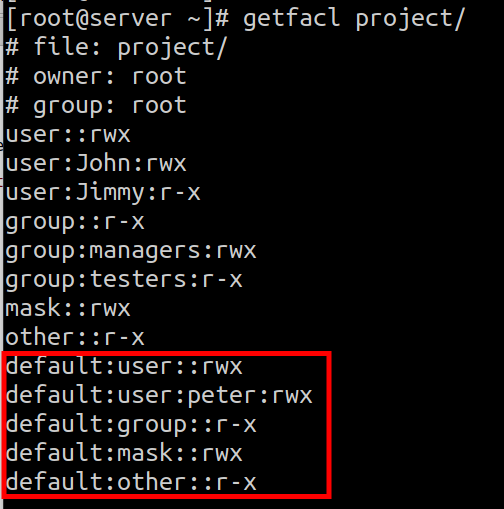
\includegraphics[scale=0.4]{content/chapter6/images/getfacl2.png}
		\caption{Sample output}
		\label{fig:acl_example2}
	\end{figure}
	

\newpage

\textbf{Remove ACL permission}
\bigskip
\begin{itemize}
	\item Syntax to remove ACL rule applied for user and group from file or directory:
	\bigskip
	\begin{tcolorbox}[breakable,notitle,boxrule=-0pt,colback=pink,colframe=pink]
		\color{black}
		\fontdimen2\font=0.5em
		Syntax: setfacl -x u:user\_name file\_or\_directory
		\newline
		Syntax: setfacl -x g:group\_name file\_or\_directory
		\fontdimen2\font=4pt
	\end{tcolorbox}
	Eg: Remove ACL rule for file named \textbf{secretfile} for user \textbf{john}:
	\begin{tcolorbox}[breakable,notitle,boxrule=-0pt,colback=black,colframe=black]
		\color{green}
		\fontdimen2\font=9pt
		\# setfacl -x u:john secretfile
		\fontdimen2\font=4pt
	\end{tcolorbox}

\bigskip
\bigskip

	\item Syntax to remove default ACL rule applied for user and group from a directory:
	\bigskip
	\begin{tcolorbox}[breakable,notitle,boxrule=-0pt,colback=pink,colframe=pink]
		\color{black}
		\fontdimen2\font=0.5em
		Syntax: setfacl -R -x u:user\_name directory
		\newline
		Syntax: setfacl -R -x g:group\_name directory
		\fontdimen2\font=4pt
	\end{tcolorbox}
	Eg: Remove ACL rule on \textbf{project} directory for user \textbf{john}:
	\bigskip
	\begin{tcolorbox}[breakable,notitle,boxrule=-0pt,colback=black,colframe=black]
		\color{green}
		\fontdimen2\font=9pt
		\# setfacl -R -x u:john project
		\fontdimen2\font=4pt
	\end{tcolorbox}
		
\end{itemize}

\end{itemize}

\end{flushleft}

\newpage

